

$$
\left[ \begin{array}{l}
    \dfrac{dv}{du} = \dfrac{\lambda_2}{\lambda_1} \cdot \dfrac{u}{v}\\
    u = 0
\end{array} \right.
\Longleftarrow
\begin{cases}
    \dot{u} = \lambda_1 u \\
    \dot{v} = \lambda_2 v
\end{cases} \Longrightarrow
\begin{cases}
    u = c_1 \cdot e^{\lambda_1 t}\\
    v = c_2 \cdot e^{\lambda_2 t}
\end{cases}
$$
Поділили двуге рівняння на перше, щоб вилучити $t$.
$$
\left[ \begin{array}{l}
    \dfrac{dv}{du} = \dfrac{\lambda_2}{\lambda_1} \cdot \dfrac{u}{v}\\
    u = 0
\end{array} \right. \Longrightarrow \left[ \begin{array}{l}
    \ln{ \left| v \right| } = \dfrac{\lambda_2}{\lambda_1} \ln{ \left| u \right| } + \ln{ \left| c \right| } \\
    u = 0, v = 0
\end{array} \right. \Longrightarrow
\left[ \begin{array}{l}
    v = c  \cdot u^{ \frac{\lambda_2}{\lambda_1} }\\
    u = 0, v = 0
\end{array} \right.
$$

Якщо $ \lambda_1 \cdot \lambda_1 > 0 $ та $ \left| \lambda_2 \right| > \left| \lambda_1 \right|  $ (стрілки від нуля за умови $
 \lambda_1, \lambda_2 > 0$):

\begin{center} 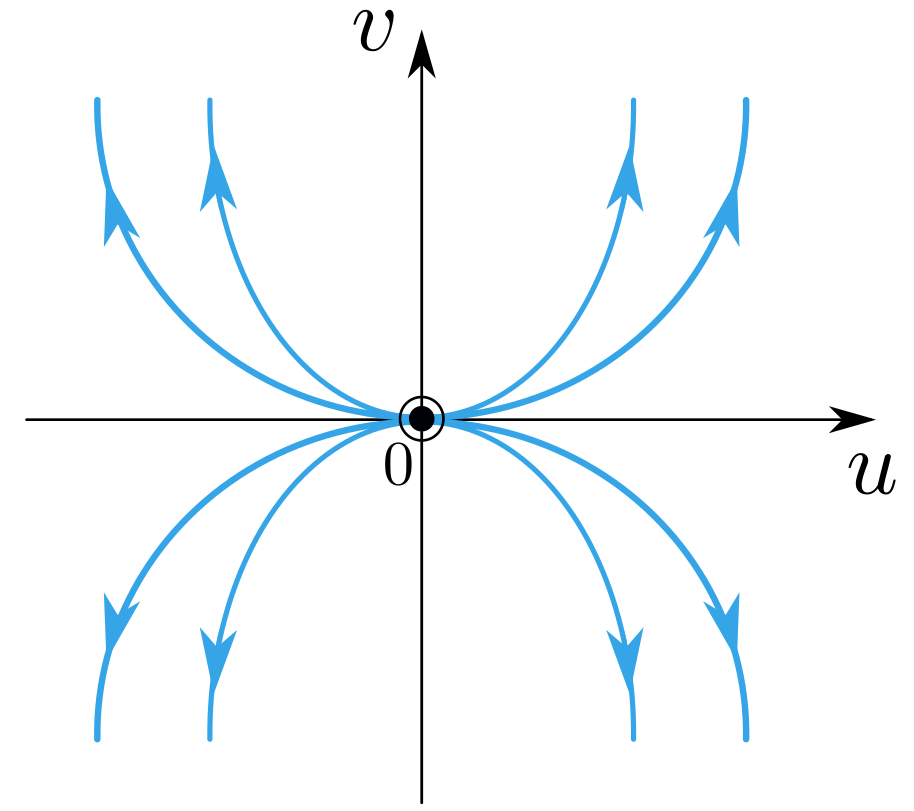
\includegraphics[scale=0.3]{assets/lectures_recent-b13d607a.png} \end{center}

Якщо $ \lambda_2 \cdot \lambda_1 > 0$ та  $ \left| \lambda_2 \right| > \left| \lambda_1 \right|  $ (стрілки до нуля за умови $
 \lambda_1, \lambda_2 < 0$):

 \begin{center} 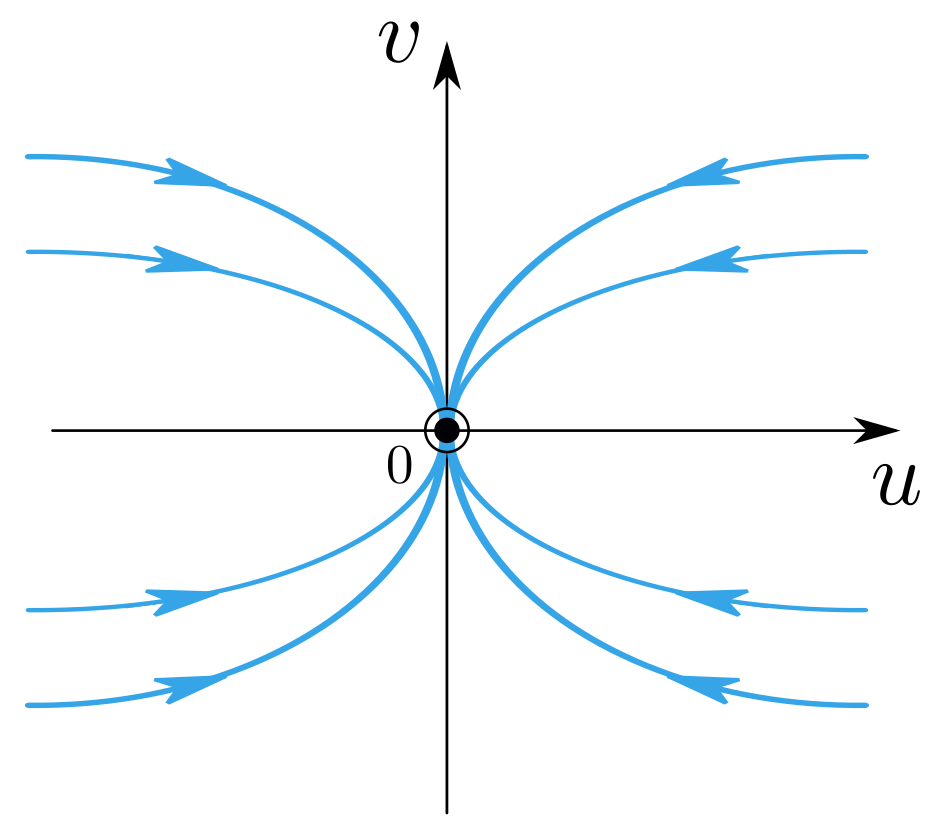
\includegraphics[scale=0.3]{assets/lectures_recent-392ff5ad.png} \end{center}

 Відмітимо, що якщо $\lambda_1, \lambda_2 < 0$, то напрям руху (по $t$) вздовж траєкторій відбувається до нуля. Якщо ж $\lambda_1, \lambda_2 >0$, то рух спрямовано від нуля.\\

 Залишається перейти до початкових змінних $ \begin{bmatrix}
  x \\
   y
 \end{bmatrix}$.\\
Таким чином, якщо $\lambda_1 , \lambda_2 \in \mathbb{R}, \lambda_1 \neq \lambda_2, \lambda_1 \cdot \lambda_2 > 0$ (власні числа одного знаку), то фазовий портрет має вигляд:

\begin{center} 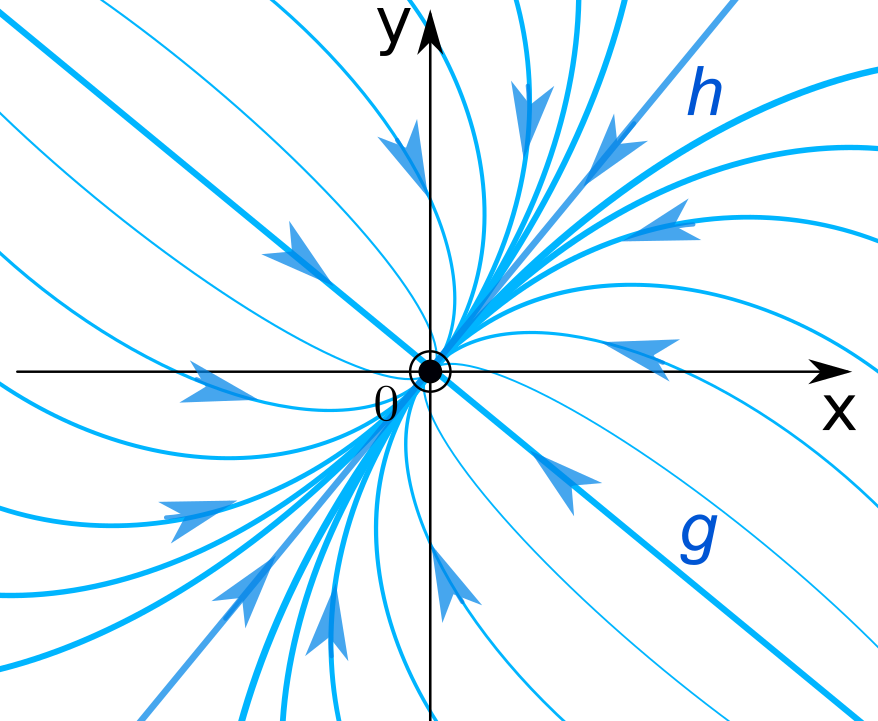
\includegraphics[scale=0.3]{assets/lectures_recent-deaf1762.png} \end{center}

На малюнку $h$ - пряма на якій лежить власний вектор, який відповідає меншому за модулем власному числу.\\
Такий фазовий портрет \textbf{вузол.}\\
- Якщо $\lambda_1, \lambda_2 > 0$ - нестійкий вузол (стрілки від нуля).\\
- Якщо $\lambda_1, \lambda_2 < 0$ - ас. стійкий вузол (стрілки до нуля).

\begin{example}
    $$
    \begin{cases}
    \dot{x} = 2y - 3x\\
    \dot{y} = x - 4y
    \end{cases} \qquad A = \begin{bmatrix}
     -3 & 2 \\
     1 & -4
    \end{bmatrix}
    $$
    $$
    \det{A - \lambda I} = \begin{vmatrix}
      -3 - \lambda & 2 \\
      1 & -4 - \lambda
    \end{vmatrix}  = (-3-\lambda) (-4 - \lambda) -2 = \lambda^2 + 7 \lambda + 10 = 0
    $$
    $$
    \lambda_1 = -2 \qquad \lambda_2 = -5 \Rightarrow \text{ас. стійкий вузол.}
    $$
    Знаходимо власні вектори:\\
    $\lambda_1 = -2$:
    $$
    \begin{bmatrix}
     -1 & 2 \\
     1 & -2
    \end{bmatrix} \begin{bmatrix}
     h_1 \\
     h_2
    \end{bmatrix} = \begin{bmatrix}
     0 \\
     0
    \end{bmatrix} \qquad \begin{gathered}
     -h_1 + 2h_2 = 0\\
     h_1 = 2 h_2
    \end{gathered} \Rightarrow \overline{h} = \begin{bmatrix}
     2 \\
     1
    \end{bmatrix}
    $$
    $\lambda_2 = -5$
    $$
    \begin{bmatrix}
     2 & 2 \\
     1 & 1
    \end{bmatrix} \begin{bmatrix}
     g_1 \\
     g_2
    \end{bmatrix} = \begin{bmatrix}
     0 \\
     0
    \end{bmatrix}
    \qquad \begin{gathered}
     g_1 + g_2 = 0\\
     g_1 = - g_2
    \end{gathered} \Rightarrow \overline{g} = \begin{bmatrix}
     1 \\
     -1
    \end{bmatrix}
    $$

    \begin{center} 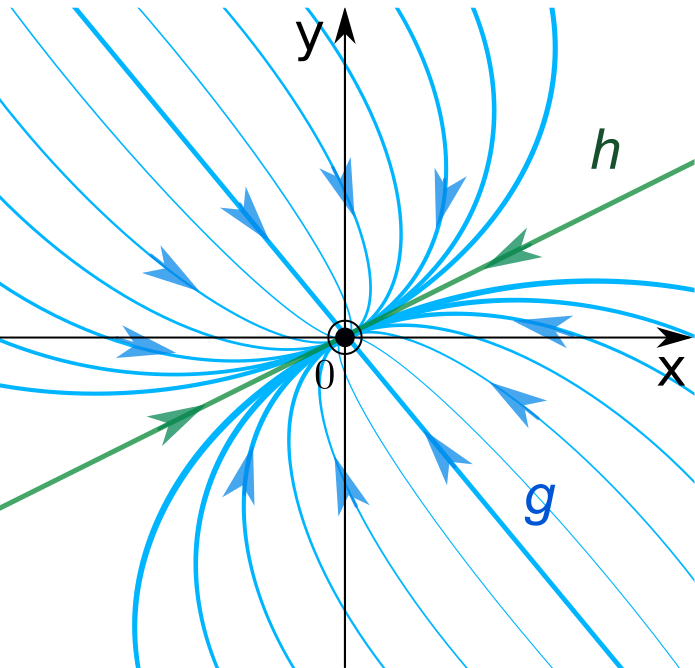
\includegraphics[scale=0.4]{assets/lectures_recent-06adae22.png} \end{center}
\end{example}

2. Нехай $ \lambda_1 , \lambda_2 \in \mathbb{R}, \lambda_1 \neq \lambda_2, \lambda_1 \cdot \lambda_2 < 0$ (Власні числа різних знаків).
Тоді, аналогічно, перейшовши до Жорданового базису, маємо:

$$
\begin{gathered}
\begin{cases}
    \dot{u} = \lambda_1 u\\
    \dot{v} = \lambda_2 v
\end{cases} \\ \begin{cases}
    u = c_1 \cdot e^{\lambda_1 t}\\
    v = c_2 \cdot e^{\lambda_2 t}
\end{cases} \\
 \left[ \begin{array}{l}
v = C \cdot u^{ \frac{\lambda_2}{\lambda_1} }\\
u =0 , v = 0
\end{array} \right.
\end{gathered}\quad
\begin{gathered} 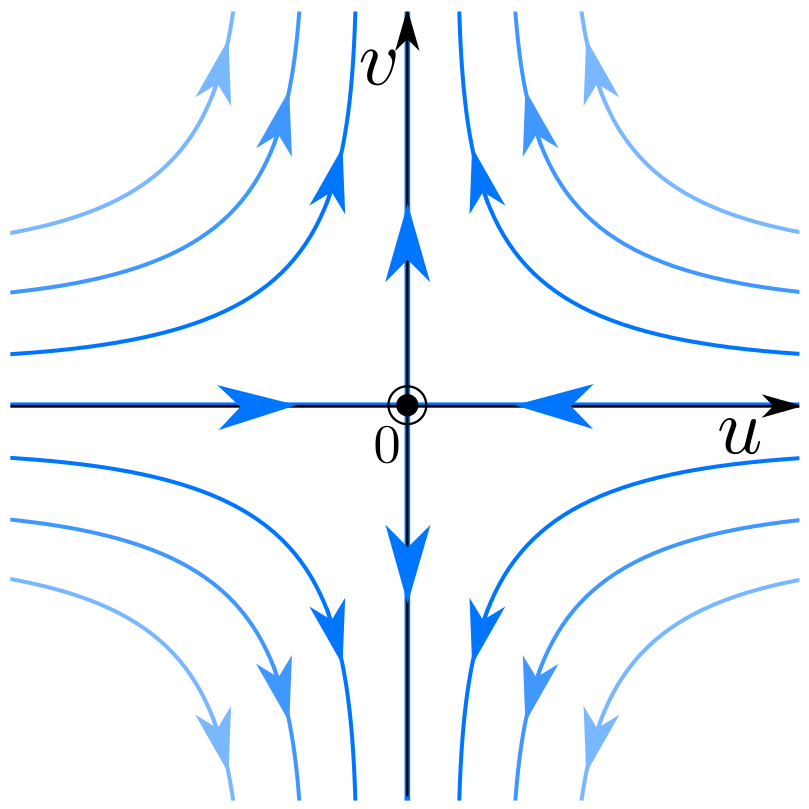
\includegraphics[scale=0.3]{assets/lectures_recent-53a0acd8.png} \end{gathered}
$$


Якщо $ \lambda_1 < 0,
  \lambda_2 > 0
$, то $
 \begin{gathered}
 u(t) \xrightarrow[t \to \infty]{} 0\\
 v(t) \xrightarrow[t \to \infty]{} \infty
 \end{gathered}.$\\
 Якщо $ \lambda_1 < 0,
  \lambda_2 > 0$, то  $
   \begin{gathered}
   u(t) \xrightarrow[t \to \infty]{} \infty\\
   v(t) \xrightarrow[t \to \infty]{} 0
   \end{gathered}.$\\
У другому випадку напрям руху траекторій відбуватиметься в інший бік.\\
Отже, перейшовши до початкових змінних, отримаємо, що за умови $\lambda_1 \cdot \lambda_2 < 0$ фазовий портрет має вигляд:

\begin{center} 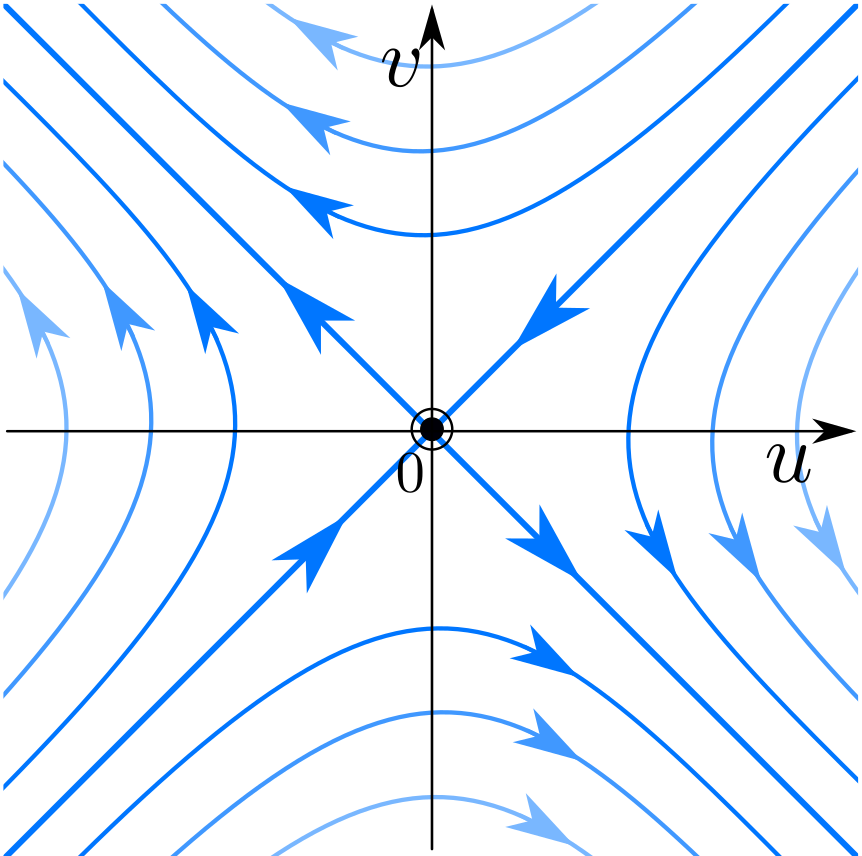
\includegraphics[scale=0.25]{assets/lectures_recent-0ebe704d.png} \end{center}

\begin{remark}
    Стрілки до нуля вздовж прямої, на якій лежить власний вектор, що відповідає $ \lambda_1 < 0$.\\
    Стрілки від нуля вздовж прямої, на якій лежить власний вектор, що відповідає $ \lambda_2 > 0$.
\end{remark}
Такий фазовий портрет називається \textbf{сідло}. Це завжди нестійке положення рівноваги.

\begin{example}
    $$
    \begin{cases}
        \dot{x} = x + 3y\\
        \dot{y} = 2x
    \end{cases} \qquad A = \begin{bmatrix}
     1 & 3 \\
     2 & 0
    \end{bmatrix}
    $$
    $$
    \det (A - \lambda I) = \begin{vmatrix}
      1-\lambda & 3 \\
      2 & - \lambda
    \end{vmatrix} = (1- \lambda)(-\lambda) - 6 = \lambda^2 - \lambda - 6 = 0
    $$
    $$
    \lambda_1 = 3 \quad \lambda_2 = -2 \Longrightarrow \text{сідло (нестійке)}
    $$
    Знаходимо власні вектори:
    $\lambda_1 = 3$
    $$
    \begin{bmatrix}
     -2 & 3\\
     2 & -3
    \end{bmatrix} \begin{bmatrix}
     h_1\\
     h_2
    \end{bmatrix} = \begin{bmatrix}
      0\\
      0
    \end{bmatrix} \qquad 2h_1 = 3 h_2 \Rightarrow \overline{h} = \begin{bmatrix}
     3 \\
     2
    \end{bmatrix}
    $$

    $\lambda_2 = -2$

    $$
    \begin{bmatrix}
     3 &3 \\
     2 & 2
    \end{bmatrix} \begin{bmatrix}
     g_1 \\
     g_2
    \end{bmatrix} = \begin{bmatrix}
     0 \\
     0
    \end{bmatrix} \qquad 2 g_1 =-2 g_2 \Rightarrow \overline{g} = \begin{bmatrix}
     1 \\
     -1
    \end{bmatrix}
    $$
    Отримали такий фазовий портрет:
    \begin{center} 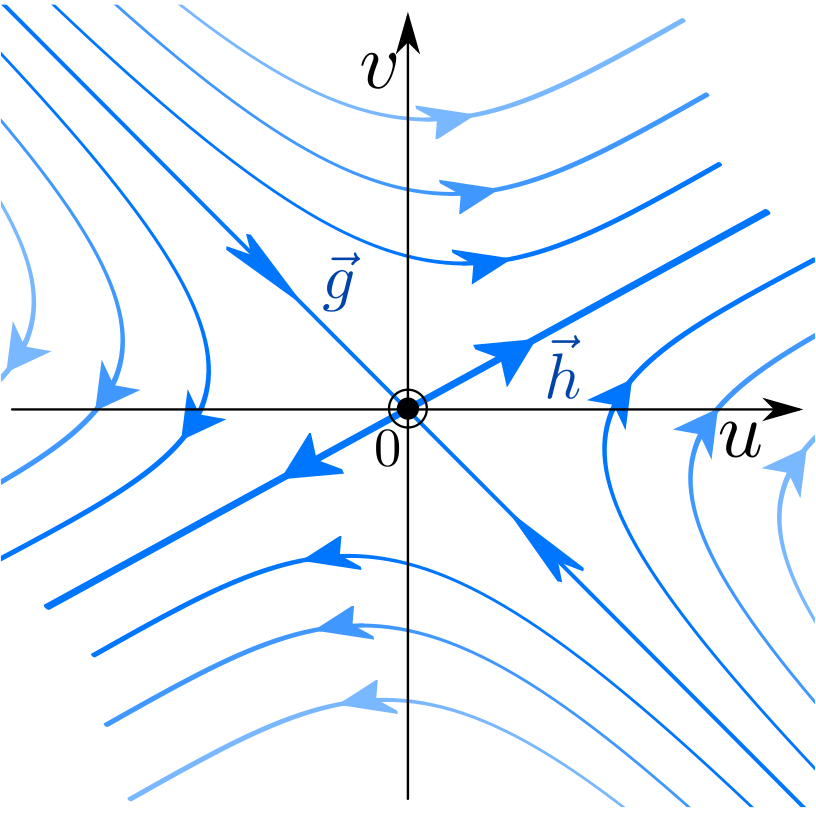
\includegraphics[scale=0.3]{assets/lectures_recent-c4b9c37b.png} \end{center}
    \end{example}


    3. Нехай $ \lambda_1 = \lambda_2 = \lambda \in \mathbb{R}$.\\
    a) Матриця $A$ - діагональна.
    $$
    A = \begin{bmatrix}
     \lambda & 0 \\
     0 & \lambda
    \end{bmatrix} \Longrightarrow \begin{cases}
        \dot{x} = \lambda x\\
        \dot{y} = \lambda y
    \end{cases}
    $$
    В такому випадку, фазовий портрет називають \textbf{диктричний вузол.}




\begin{center} 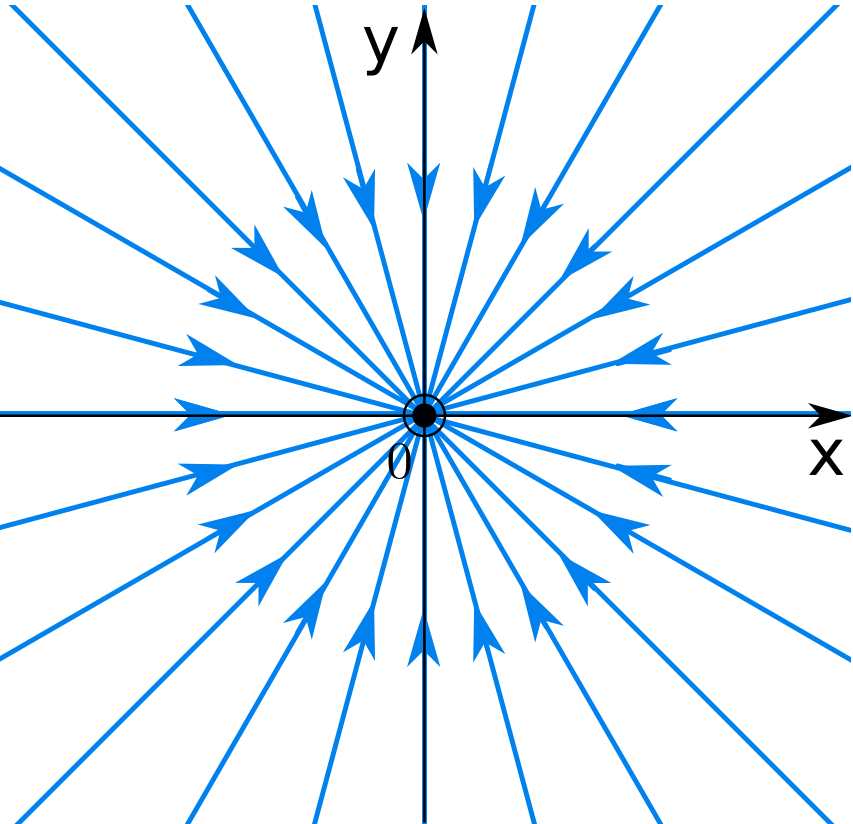
\includegraphics[scale=0.3]{assets/lectures_recent-ab36e3f3.png} \end{center}


Якщо $ \lambda < 0 $ - ас. стійкий (стрілки до нуля).\\
Якщо $ \lambda > 0 $ - нейстійкий (стрілки від нуля). \\
б) Матриця $A$ - недіагональна. В такому разі, фазовий портрет називають \textbf{вироджений вузол.}\\
- якщо $ \lambda < 0 $ - ас. стійкий ( стрілки до нуля ).\\
- якщо $ \lambda > 0 $ - нестійкий (стрілки від нуля).\\
Вироджений вузол може бути двох видів:
\begin{center} 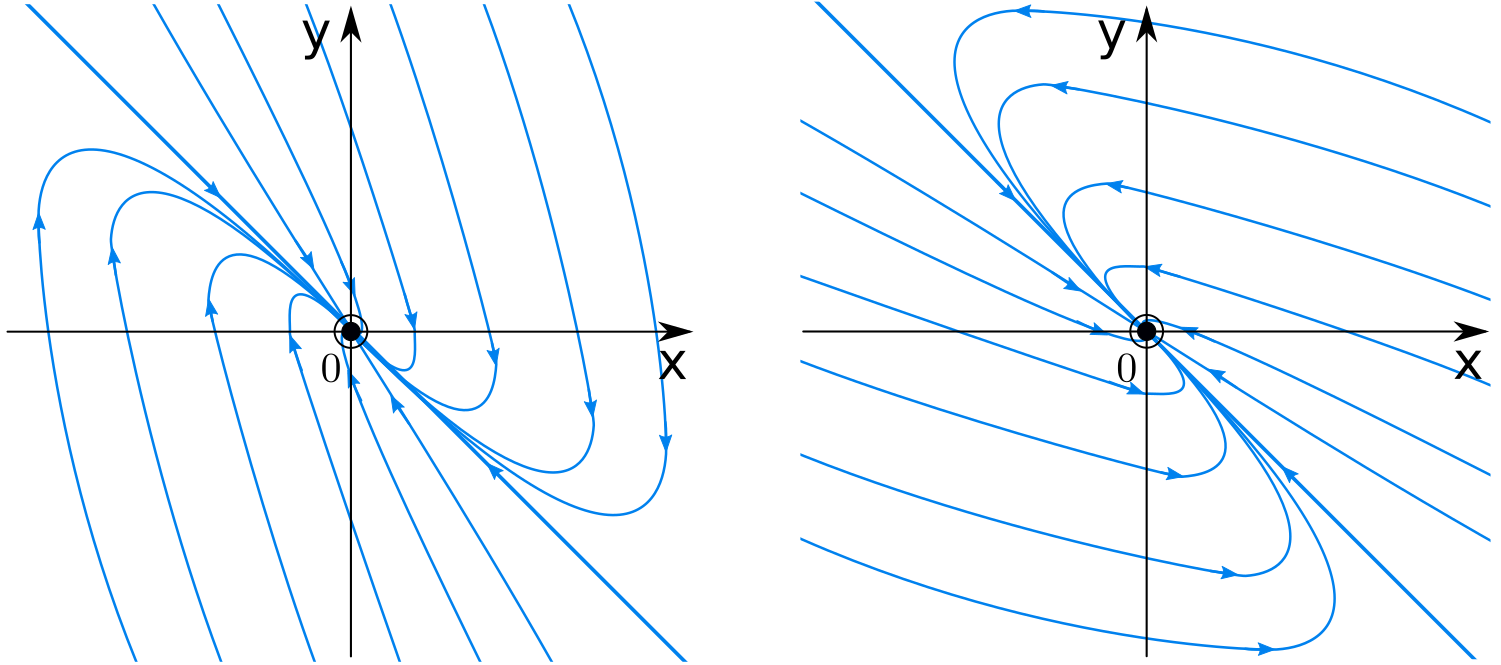
\includegraphics[scale=0.25]{assets/lectures_recent-b526bf37.png} \end{center}

Для визначення типу виродженого вузла потрібно визнгачити напрям вектора фазової швидкості $ \begin{bmatrix}
 \vec{x} \\
 \vec{y}
\end{bmatrix}$ в довільній точці, що не дорівнює нулю системи координат. Цей напрям має співпадати із напрямами руху по фазовій траєкторії (до нуля або від нуля).

\begin{example}
    $$
    \begin{cases}
        \vec{x} = 2y - 3x\\
        \vec{y} = y - 2x
    \end{cases} \qquad A = \begin{bmatrix}
     -3 & 2 \\
     -2 & 1
    \end{bmatrix}
    $$

    $$
    \det{ \left( A - \lambda I  \right) } = \begin{vmatrix}
      -3 - \lambda & 2 \\
      -2 & 1 - \lambda
    \end{vmatrix} = ( -3 - \lambda ) ( 1 -\lambda) + 4 =  \lambda^2 + 2 \lambda + 1 =
    $$
    $$
    = ( \lambda+ 1) ^2 = 0 \Longrightarrow  \lambda = -1 - \text{кратності 2. }
    $$
З попереднього випливає, що фазовим портретом буде асимптотично стійкий вироджений вузол (стрілки до нуля).
Знайдемо власний вектор:
$$
\begin{bmatrix}
 -2 & 2 \\
 2 & 2
\end{bmatrix} \begin{bmatrix}
 h_1 \\
 h_2
\end{bmatrix} = \begin{bmatrix}
 0 \\
 0
\end{bmatrix} \qquad h_1 = h_2 \Rightarrow \overline{h} = \begin{bmatrix}
 1 \\
 1
\end{bmatrix}
$$

\begin{center} 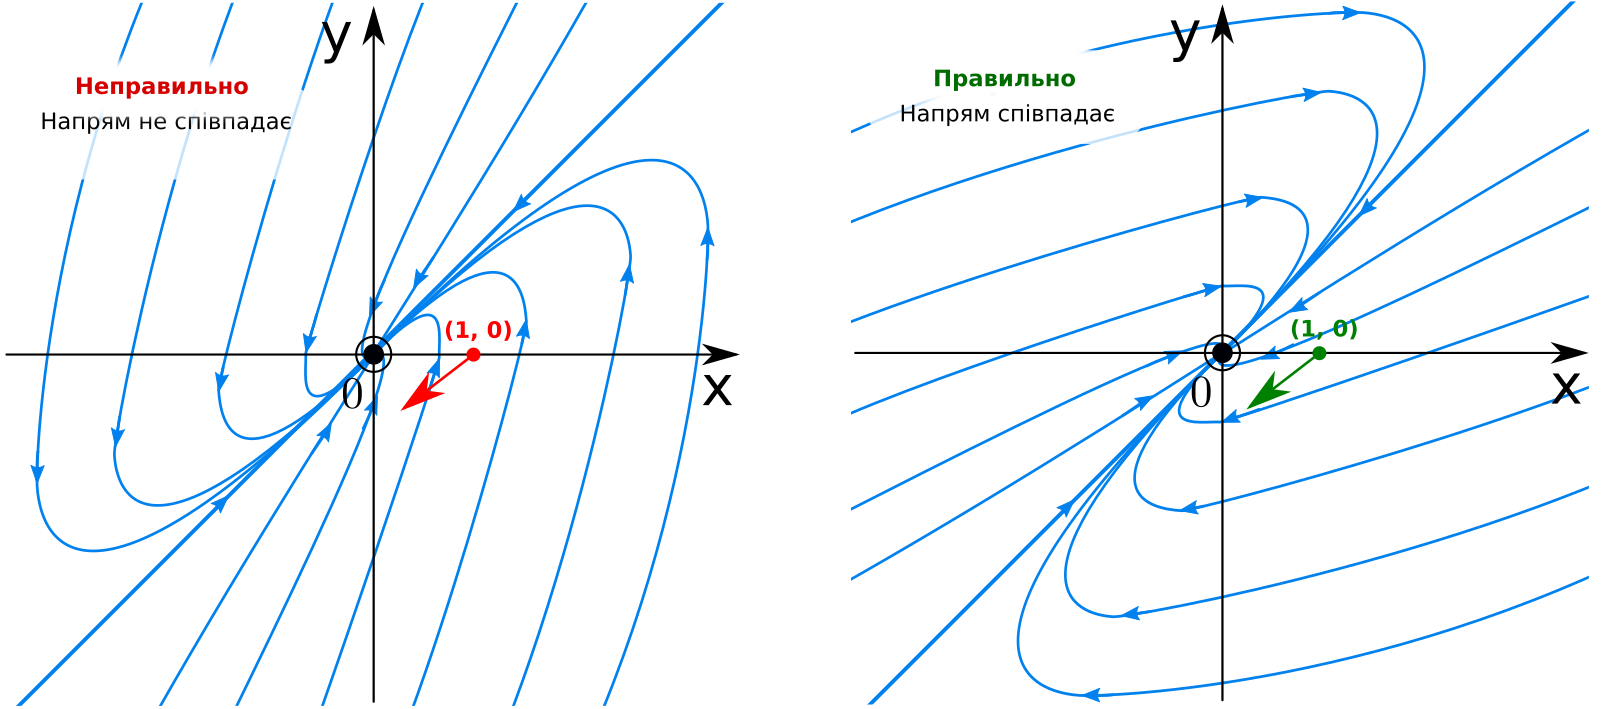
\includegraphics[scale=0.3]{assets/lectures_recent-f0de3cfc.png} \end{center}

Візьмемо т. (1, 0):
$$
\begin{bmatrix}
 \dot{x} \\
 \dot{y}
\end{bmatrix} \Bigg|_{(1,0)} = \begin{bmatrix}
 -3 \\
 -2
\end{bmatrix} \Longrightarrow \begin{gathered}
 x_k = -2 \\
 y_k = -2
\end{gathered}
$$

\end{example}

4. $\lambda_{1, 2} - \alpha \pm i\beta, \alpha\neq 0$. В такому випадку, фазовий портрет назвається \textbf{фокус}. Якщо $ \alpha > 0$ - нестійкий. Якщо $ \alpha > 0$ - ас. стійкий.
Фазовий портрет ''фокус'' може бути двох видів:
\begin{center} 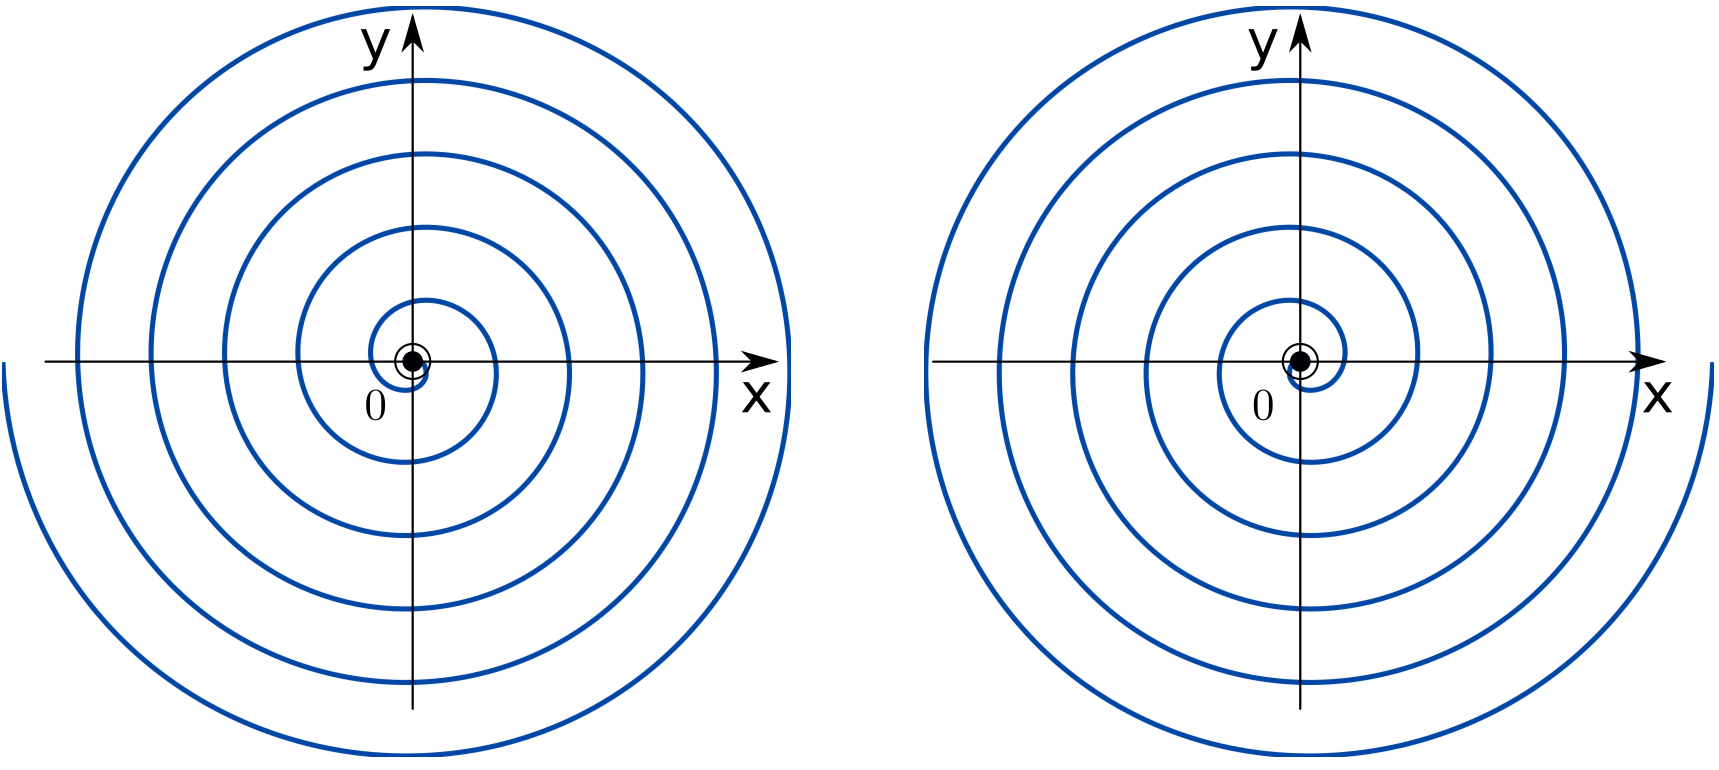
\includegraphics[scale=0.3]{assets/lectures_recent-9fe11a21.png} \end{center}
Для визначення типу фокуса визначаємо напрям вектора фазової швидкості в довільній точці, що не дорівнює нулю.

\begin{example}
    $$
    \begin{cases}
        \dot{x } = x - 2y\\
        \dot{y} = 4x - 3y
    \end{cases} \qquad A = \begin{bmatrix}
     1 & -2 \\
     4 & -3
    \end{bmatrix}
    $$
    $$ \det{(A - \lambda I)} = \begin{vmatrix}
      1- \lambda & -2 \\
      4 & -3-\lambda
    \end{vmatrix}  = ( 1- \lambda) (-3 - \lambda) + 8 = \lambda^2 + 2 \lambda + 5 = 0$$
$$
D = -16 \quad \lambda_{1,2} = \frac{-2 \pm 4i}{2} = -1 \pm 2i
$$
Асимптотично стійкий фокус (стрілки до нуля).
\begin{center} 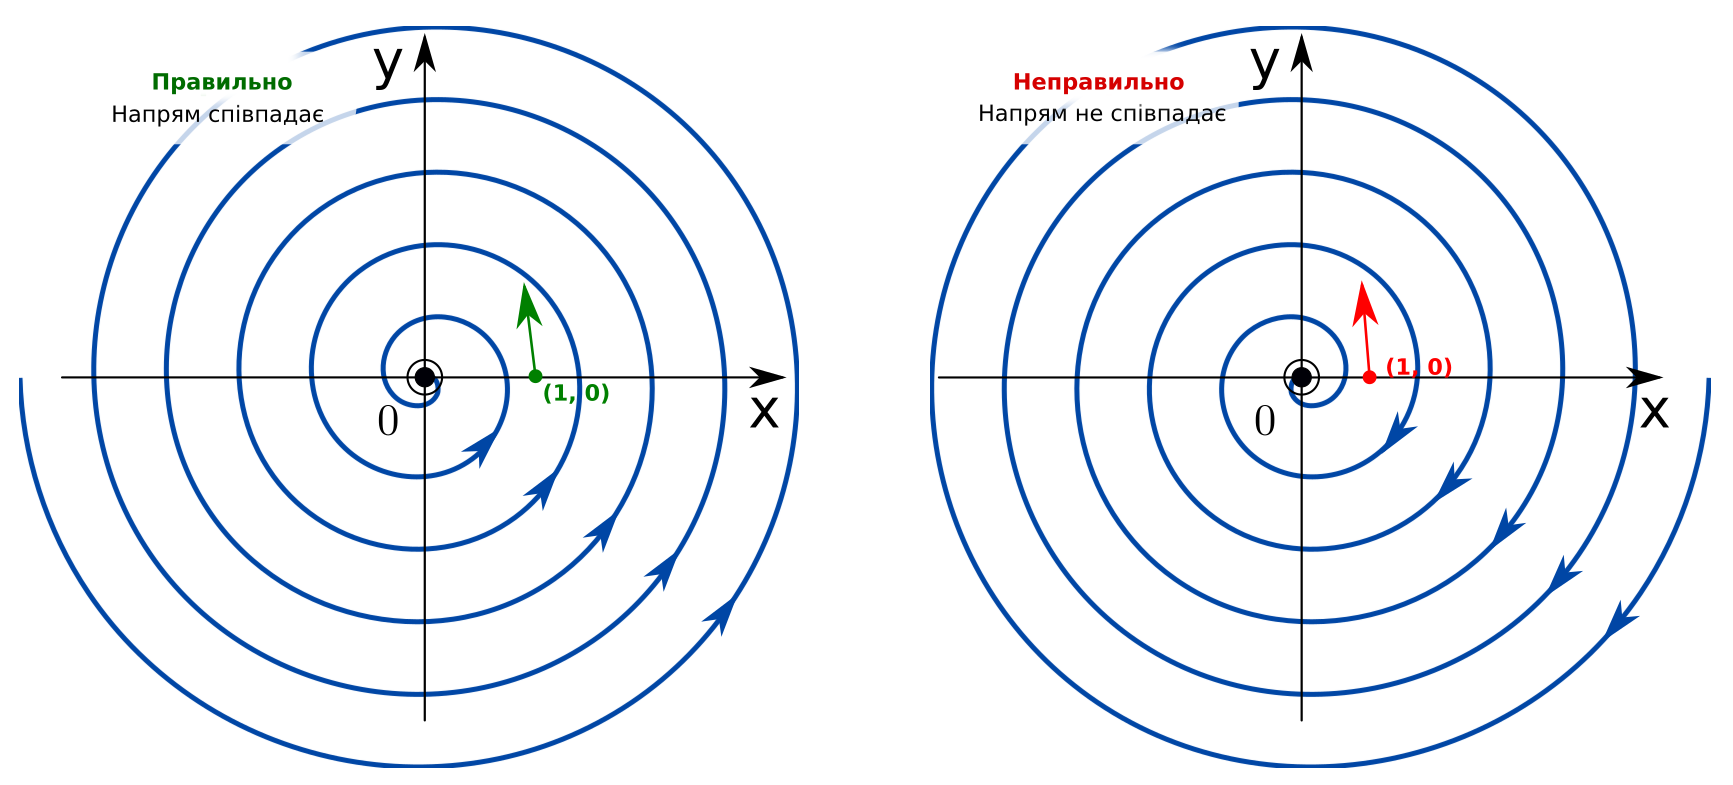
\includegraphics[scale=0.27]{assets/lectures_recent-b90426e3.png} \end{center}
Візьмемо точку (1, 0) для перевірки:

$$
\begin{bmatrix}
 \dot{x}\\
 \dot{y}
\end{bmatrix}\Bigg|_{(1,0)} - \begin{bmatrix}
 1 \\
 4
\end{bmatrix} \qquad \begin{gathered}
 x_k -1 = 1 \\
 y_k - 0 = 4
\end{gathered} \Rightarrow \begin{gathered}
 x_k = 2 \\
 y_k  = 4
\end{gathered}
$$
Отримали: $(1,0) \to (2, 4)$. Перевіримо за виглядом фазового портрета вище.
\end{example}

5.$ \lambda_{1,2} = \pm i \beta$. За таких власних чисел, фазовий портрет називається \textbf{центр.} (стійкий, але не асимптотично стійкий)
\begin{center} 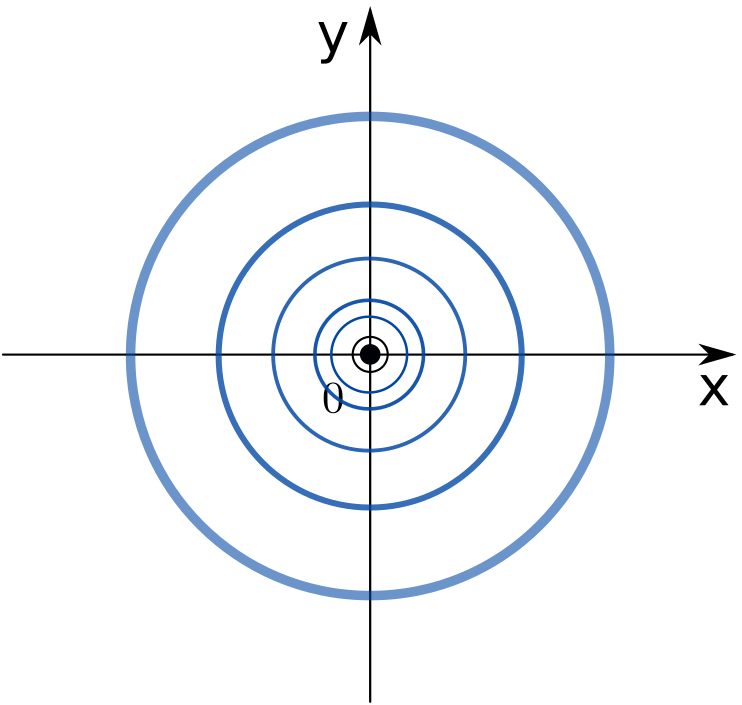
\includegraphics[scale=0.3]{assets/lectures_recent-2982f611.png} \end{center}

\begin{example}
    $$
    \begin{cases}
        \dot{x} = -2 x - 5y \\
        \dot{y} = 2x + 2y
    \end{cases} \qquad A = \begin{bmatrix}
     -2 & -5\\
     2 & 2
    \end{bmatrix}
    $$
    $$
    \det{(A - \lambda I)} = \begin{vmatrix}
      -2-\lambda & -5 \\
      2 & 2 -\lambda
    \end{vmatrix}  = \lambda^2 + 6 = 0 \Rightarrow \lambda = \pm i \sqrt{6} \Rightarrow \text{центр}
    $$
    Візьмемо т. (1, 0):
    $$
\begin{gathered}
\begin{bmatrix}
 \dot{x}\\
 \dot{y}
\end{bmatrix}\Bigg|_{(1,0)} = \begin{bmatrix}
 -2 \\
 2
\end{bmatrix} \\ \begin{cases}
  x_k -1 = -2\\
  y_k  - 0 = 2
\end{cases} \\
\begin{cases}
x_k = -1\\
    y_k  =2
\end{cases}
\end{gathered}\qquad    \begin{gathered} 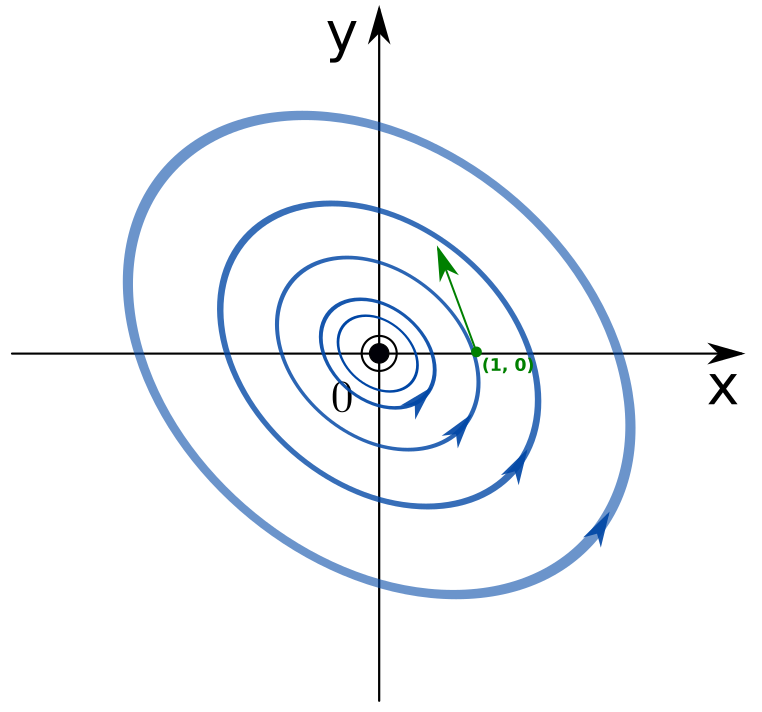
\includegraphics[scale=0.3]{assets/lectures_recent-1467e19e.png} \end{gathered}
    $$


\end{example}
6. Нехай $ \det A = 0$ (вирджений випадок).\\
$$
\det A  =  \begin{vmatrix}
  a & b\\
  c & d
\end{vmatrix} = ad - bc  = 0 \Rightarrow \frac{a}{c} = \frac{b}{d} = 0 \quad \begin{gathered}
 a = kc\\
 b = kd
\end{gathered}
$$
$$
\begin{cases}
    \dot{x} = ax+ by\\
    \dot{y} = k(ax + by)
\end{cases} \Rightarrow ax + by  = 0 \text{ - пряма положень рівноваги.}
$$

$$
\det ( A - \lambda I) = \begin{vmatrix}
  a - \lambda & b\\
  ka & kb - \lambda
\end{vmatrix} = (a-\lambda)*(kb- \lambda) - kab =
$$
$$
 = akb - a \lambda - kb \lambda +  \lambda^2 - kab = \lambda^2 - (a + kb) \lambda =0
 $$
 $$
 \lambda = 0 \qquad \lambda = a + bk
 $$

 a) Прямі паралельні власному вектору, що відповідає власному числу $\lambda =  a + bk$\\
 $\lambda > 0 $ - стрілки від нуля.\\
 $\lambda < 0 $ - стрілки до нуля.\\

 \begin{center} 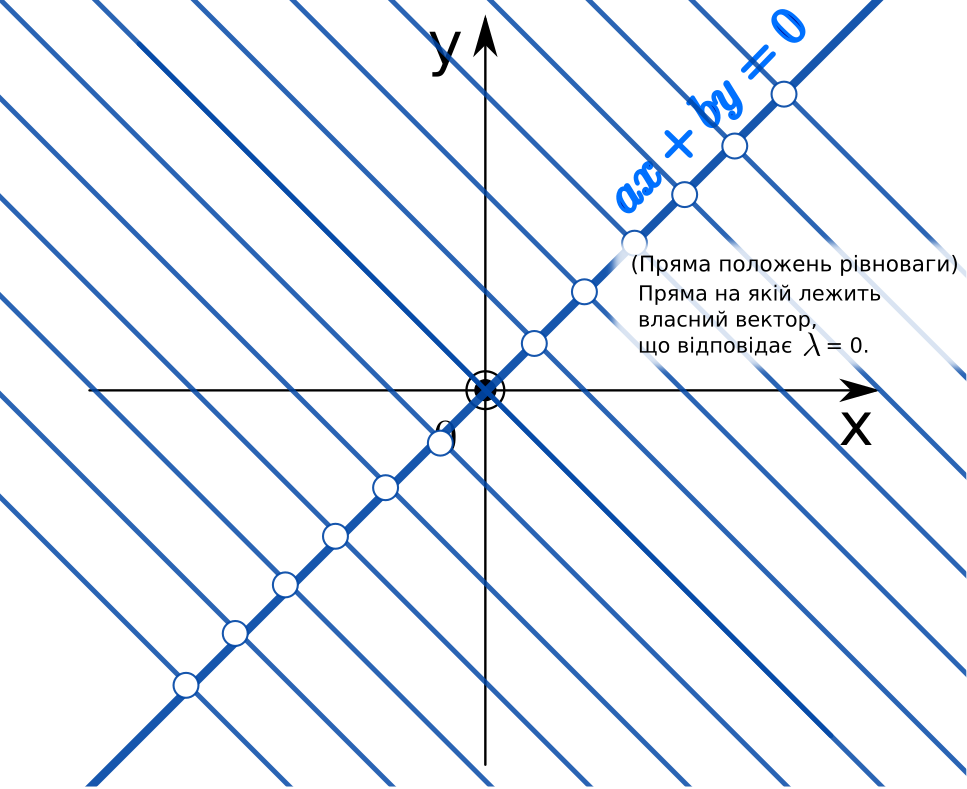
\includegraphics[scale=0.3]{assets/lectures_recent-058ceaff.png} \end{center}
b) $ \lambda_1 =  \lambda_2 = 0 \quad (a = - bk)$

\begin{center} 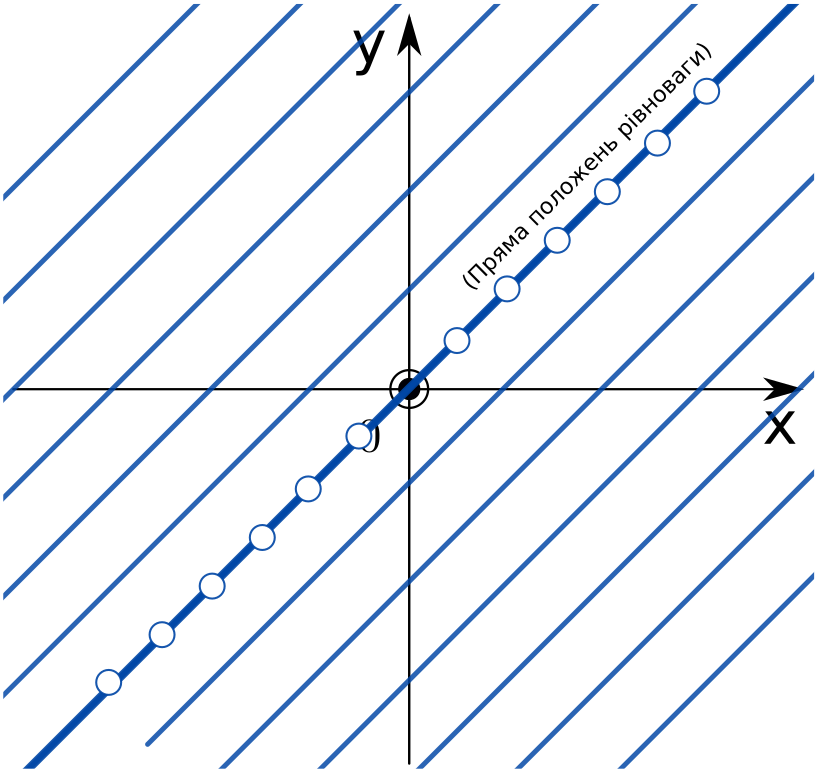
\includegraphics[scale=0.3]{assets/lectures_recent-49093f01.png} \end{center}
